\begin{thmBox}{35.1 (Tietze Extension Theorem)}[thm:35.1]
Let \( X \) be a normal space; let \( A \) be a closed subspace of \( X \)

\begin{enumerate}[label = (\alph*)]
    \item Any continuous map of \( A \) into the closed interval \( [ a, b ] \) of
        \( \mathbb{R} \) may be extended to a continuous map of all of \( X \) into
        \( [ a, b ] \). 
    \item Any continuous map of \( A \) into \( \mathbb{R} \) may be extended to a 
        continuous map of all of \( X \) into \( \mathbb{R} \). 
\end{enumerate}

\baseRule

\begin{proofBox}*
    \wrapBox{Main Idea of the Proof} 

    The idea of the proof is to construct a sequence of continuous functions 
    \( s_{ n } \) defined on the entire space \( X \), such that the sequence 
    \( s_{ n } \) converges uniformly, and such that the restriction of 
    \( s_{ n } \) to \( A \) approximates \( f \) more and more closely as 
    \( n \) becomes large. 
    Then the limit function will be continuous, and its restriction to \( A \) 
    will equal \( f \). 
    
    \baseSkip
    \wrapBox{Step 1} 

    The first step is to construct a particular function \( g \) defined on all of
    \( X \) such that \( g \) is not too large, and such that \( g \) approximates
    \( f \) on the set \( A \) to a fair degree of accuracy. 
    To be more precise, let us take the case \( f: A \rightarrow [ -r, r ] \). 
    We assert that there exists a continuous function 
    \( g: X \rightarrow \mathbb{R} \) such that 
    \begin{equation*}
        \begin{alignedat}{2}
            \lvert g ( x ) \rvert &\leq \frac{ 1 }{ 3 } r 
            &&\quad \forall x \in X
            \\
            \lvert g ( a ) - f ( a ) \rvert &\leq \frac{ 2 }{ 3 } r 
            &&\quad \forall a \in A 
        \end{alignedat}
    \end{equation*}
    The function \( g \) is constructed as follows: 
    Divide the interval \( [ -r, r ] \) into three equal intervals of length
    \( \frac{ 2 }{ 3 } r \):
    \begin{equation*}
        I_{ 1 }
        =
        [ -r, -\tfrac{ 1 }{ 3 } r ]
        \quad 
        I_{ 2 }
        =
        [ - \tfrac{ 1 }{ 3 }r, \tfrac{ 1 }{ 3 }r ]
        \quad 
        I_{ 3 }
        =
        [ \tfrac{ 1 }{ 3 } r, r ]
    \end{equation*}
    Let \( B \) and \( C \) be the subsets
    \begin{equation*}
        B = f^{ -1 } ( I_{ 1 } )
        \quad \mathrm{and} \quad 
        C = f^{ -1 } ( I_{ 3 } )
    \end{equation*}
    of \( A \). Because \( f \) is continuous, we see that 
    \begin{equation*}
        I_{ 1 } \cap I_{ 3 }
        =
        \emptyset
        \implies
        f^{ -1 } ( I_{ 1 } \cap I_{ 3 } ) = f^{ -1 } ( \emptyset )
        \iff 
        f^{ -1 } ( I_{ 1 } ) \cap f^{ -1 } ( I_{ 3 } ) = \emptyset
    \end{equation*}
    which tells us that \( B \) and \( C \) are closed disjoint subset of \( A \). 
    Since \( A \) is given to be a closed subspace of \( X \), we see by the 
    transitivity of closed sets that \( B \) and \( C \) are also disjoint closed 
    subsets of \( X \). 

    \baseSkip

    By the [\hyperlink{thm33.1}{Urysohn Lemma}], we see that there exists a 
    continuous function 
    \begin{equation*}
        g: X \rightarrow [ - \tfrac{ 1 }{ 3 } r, \tfrac{ 1 }{ 3 } r ]
    \end{equation*}
    having the property that \( g ( x ) = - \frac{ 1 }{ 3 } r \) for each 
    \( x \in B \), and \( g ( x ) = \frac{ 1 }{ 3 } r \) for each \( x \in C \). 
    Then, we have that \( \lvert g ( x ) \rvert \leq \frac{ 1 }{ 3 } r \) for all
    \( x \in X \). 

    \baseSkip 

    From here, we claim that for each \( a \in A \)
    \begin{equation*}
        \lvert g ( a ) - f ( a ) \rvert \leq \frac{ 2 }{ 3 } r
    \end{equation*}
    There are three cases. 
    If \( a \in B \), then we have that 
    \begin{equation*}
        g ( a ) = - \frac{ 1 }{ 3 } r
        \quad \mathrm{and} \quad 
        f ( a ) \in I_{ 1 } \implies - r \leq f ( a ) \leq - \frac{ 1 }{ 3 } r
    \end{equation*}
    If \( a \in C \), then we have that 
    \begin{equation*}
        g ( a ) = \frac{ 1 }{ 3 } r
        \quad \mathrm{and} \quad 
        f ( a ) \in I_{ 3 } \implies \frac{ 1 }{ 3 } r \leq f ( a ) \leq r
    \end{equation*}
    If \( a \notin B \cup C \), then we have that both \( g ( a ) \) and 
    \( f ( a ) \) are in \( I_{ 2 } \), which results in 
    \begin{equation*}
        - \frac{ 1 }{ 3 } r \leq g ( a ) \leq \frac{ 1 }{ 3 } r
        \quad \mathrm{and} \quad 
        - \frac{ 1 }{ 3 } r \leq f ( a ) \leq \frac{ 1 }{ 3 } r
    \end{equation*}
    In either case, we see that 
    \( \lvert g ( a ) - f ( a ) \rvert \leq \frac{ 2 }{ 3 } r \) -- see 
    Figure (\ref{fig:35.1}).

    \begin{figure}[H]
        \centering
        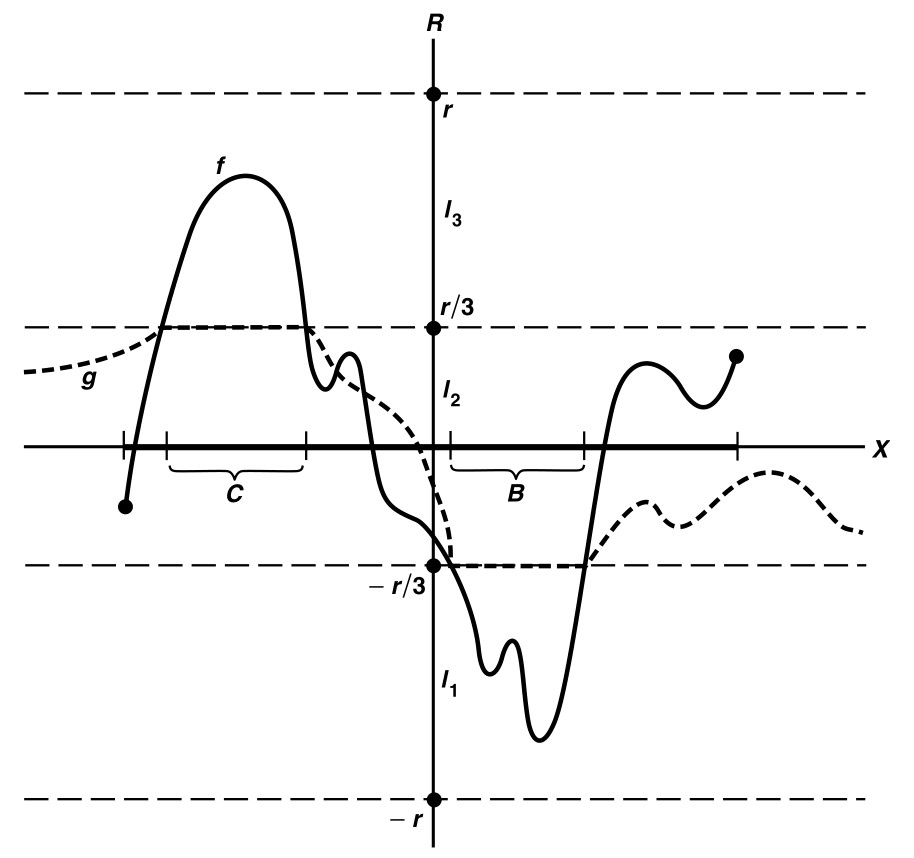
\includegraphics[ width = 0.5\linewidth ]{figures/Section 35/thm35-1.jpg}
        \caption{}
        \label{fig:35.1}
    \end{figure}

    \wrapBox{Step 2}

    We now prove part (a) of the Tietze theorem. 
    WLOG, we can replace the arbitrary closed interval \( [ a, b ] \) of
    \( \mathbb{R} \) by the interval \( [ -1, 1 ] \). 

    \baseSkip

    Let \( f: X \rightarrow [ -1, 1 ] \) be a continuous map. 
    Then \( f \) satisfies the hypotheses of Step 1, with \( r = 1 \). 
    Therefore, we have that there exists a continuous real-valued function 
    \( g_{ 1 } \), defined on all of \( X \), such that 
    \begin{equation*}
        \begin{alignedat}{2}
            \lvert g_{ 1 } ( x ) \rvert &\leq \frac{ 1 }{ 3 } 
            &&\quad \forall x \in X
            \\
            \lvert f ( a ) - g_{ 1 } ( a ) \rvert &\leq \frac{ 2 }{ 3 }
            &&\quad \forall a \in A 
        \end{alignedat}
    \end{equation*}
    Now consider the function \( f - g_{ 1 } \). 
    This function maps \( A \) into the interval 
    \( [ -\frac{ 2 }{ 3 }, \frac{ 2 }{ 3 } ] \), so we can apply Step 1 again, 
    letting \( r = \frac{ 2 }{ 3 } \). 
    We obtain a real-valued function \( g_{ 2 } \) defined on all of \( X \)
    such that 
    \begin{equation*}
        \begin{alignedat}{2}
            \lvert g_{ 2 } ( x ) \rvert &\leq 
            \frac{ 1 }{ 3 } \left( \frac{ 2 }{ 3 } \right) 
            &&\quad \forall x \in X
            \\
            \lvert f ( a ) - g_{ 1 } ( a ) - g_{ 2 } ( a ) \rvert 
            &\leq 
            \left( \frac{ 2 }{ 3 } \right)^{ 2 }
            &&\quad \forall a \in A 
        \end{alignedat}
    \end{equation*}
    Then we apply Step 1 to the function \( f - g_{ 1 } - g_{ 2 } \). And so on. 

    \baseSkip 

    At the general step, we have the real-valued function 
    \( g_{ 1 } , \ldots , g_{ n } \) defined on all of \( X \) such that 
    \begin{equation*}
        \lvert f ( a ) - g_{ 1 } ( a ) - \ldots - g_{ n } ( a ) \rvert
        \leq 
        \left( \frac{ 2 }{ 3 } \right)^{ n }
    \end{equation*}
    for \( a \in A \). 
    Applying Step 1 to the function \( f - g_{ 1 } - \ldots - g_{ n } \), with 
    \( r = ( \frac{ 2 }{ 3 } )^{ n } \), we obtain a real-valued function 
    \( g_{ n + 1 } \) defined on all of \( X \) such that 
    \begin{equation*}
        \begin{alignedat}{2}
            \lvert g_{ n + 1 } ( x ) \rvert &\leq 
            \frac{ 1 }{ 3 } \left( \frac{ 2 }{ 3 } \right)^{ n }
            &&\quad \forall x \in X
            \\
            \lvert f ( a ) - g_{ 1 } ( a ) - \ldots - g_{ n } ( a ) 
            - g_{ n + 1 } ( a ) \rvert 
            &\leq 
            \left( \frac{ 2 }{ 3 } \right)^{ n + 1 }
            &&\quad \forall a \in A 
        \end{alignedat}
    \end{equation*}
    By induction, the functions \( g_{ n } \) are defined for all \( n \). 

    \baseSkip 

    We now define 
    \begin{equation*}
        g ( x )
        =
        \sum_{ n = 1 }^{ \infty } g_{ n } ( x )
    \end{equation*}
    for all \( x \in X \). 
    We can see with how each \( g_{ n } \) is defined that this infinite series 
    converges; this follows from the comparison theorem of calculus, where 
    it converges by comparison with the geometric series 
    \begin{equation*}
        \frac{ 1 }{ 3 } 
        \sum_{ n = 1 }^{ \infty } \left( \frac{ 2 }{ 3 } \right)^{ n - 1 }
    \end{equation*}
    To show that \( g \) is continuous, we must show that the sequence 
    \begin{equation*}
        s_{ n } ( x ) = \sum_{ i = 1 }^{ n } g_{ i } ( x )
    \end{equation*}
    converges to \( g ( x ) \) uniformly for all \( x \in X \).
    This fact follows at once from the "Weierstrass \( M \)-test" of analysis. 
    Without assuming this result, one can simply note that if \( k > n \), then
    \begin{equation*}
        \begin{aligned}
            \lvert s_{ k } ( x ) - s_{ n } ( x ) \rvert
            &=
            \left\lvert
                \sum_{ i = n + 1 }^{ k } g_{ i } ( x )
            \right\rvert
            \\
            &\leq 
            \frac{ 1 }{ 3 } \sum_{ i = n + 1 }^{ k } 
            \left( \frac{ 2 }{ 3 } \right)^{ i - 1 }
            \\
            &< 
            \frac{ 1 }{ 3 } \sum_{ i = n + 1 }^{ \infty } 
            \left( \frac{ 2 }{ 3 } \right)^{ i - 1 }
            =
            \left( \frac{ 2 }{ 3 } \right)^{ n }
        \end{aligned}
    \end{equation*} 
    Holding \( n \) fixed and letting \( k \rightarrow \infty \), we see that 
    \begin{equation*}
        \lvert g ( x ) - s_{ n } ( x ) \rvert \leq 
        \left( \frac{ 2 }{ 3 } \right)^{ n }
    \end{equation*}
    for all \( x \in X \). 
    Therefore, we see that \( s_{ n } \) converges to \( g \) uniformly. 

    \baseSkip 

    We now want to show that \( g ( a ) = f ( a ) \) for all \( a \in A \) -- that 
    is, we want to show that the restriction of \( g \) to \( A \) equals \( f \).
    Let 
    \begin{equation*}
        s_{ n } ( x ) = \sum_{ i = 1 }^{ n } g_{ i } ( x )
    \end{equation*}
    be the \( n \)th partial sum of the series. 
    Then \( g ( x ) \) is by definition the limit of the infinite sequence 
    \( s_{ n } ( x ) \) of partial sums, as we have shown earlier. 
    Since 
    \begin{equation*}
        \left\lvert
            f ( a ) - \sum_{ i = 1 }^{ n } g_{ i } ( a )
        \right\rvert
        =
        \lvert f ( a ) - s_{ n } ( a ) \rvert
        \leq 
        \left( \frac{ 2 }{ 3 } \right)^{ n }
    \end{equation*}
    for all \( a \in A \), it follows that \( s_{ n } \rightarrow f ( a ) \) 
    for all \( a \in A \). 
    Therefore, we have that \( f ( a ) = g ( a ) \) for all \( a \in A \). 

    \baseSkip 

    Finally, we want to show that \( g \) maps \( X \) into the interval 
    \( [ -1, 1 ] \). 
    This condition is in fact satisfied automatically, since we have already shown 
    earlier that \( g ( x ) \) converges for all \( x \in X \) by the comparison 
    theorem of calculus -- that is, we have 
    \begin{equation*}
        \lvert g ( x ) \rvert 
        \leq 
        \frac{ 1 }{ 3 } \sum_{ n = 1 }^{ \infty } 
        \left( \frac{ 2 }{ 3 } \right)^{ n - 1 }
        =
        1
    \end{equation*}
    However, this is just a lucky accident rather than an essential part of the 
    proof. 
    If all we knew was that \( g \) mapped \( X \) into \( \mathbb{R} \), then 
    the map \( r \circ g \), where \( r: \mathbb{R} \rightarrow [ -1, 1 ] \) is the 
    map 
    \begin{equation*}
        \begin{alignedat}{2}
            r ( y ) &= y &&\quad \text{if } \lvert y \rvert \leq 1 
            \\
            r ( y ) &= \frac{ y }{ \lvert y \rvert } 
            &&\quad \text{if } \lvert y \rvert \geq 1 
        \end{alignedat}
    \end{equation*}
    would be an extension of \( f \) mapping \( X \) into \( [ -1, 1 ] \). 

    \baseSkip 
    \wrapBox{Step 3}

    We now prove part (b) of the theorem, in which \( f \) maps \( A \) into 
    \( \mathbb{R} \). 
    We can replace \( \mathbb{R} \) by the open interval \( ( -1, 1 ) \), since 
    this interval is homeomorphic to \( \mathbb{R} \). 

    \baseSkip 

    Let \( f \) be a continuous map from \( A \) into \( ( -1, 1 ) \). 
    The half of the Tietze theorem already proved shows that we can extend 
    \( f \) to a continuous map \( g: X \rightarrow [ -1, 1 ] \) mapping 
    \( X \) into the \textit{closed} interval. 
    How can we find a map \( h \) carrying \( X \) into the \textit{open} 
    interval?

    \baseSkip 

    Given \( g \), let us define a subset \( D \) of \( X \) by the equation 
    \begin{equation*}
        D
        =
        g^{ -1 } ( \{ -1 \} ) \cup g^{ -1 } ( \{ 1 \} )
    \end{equation*}
    Since \( g \) is continuous, we have that \( D \) is the finite union of 
    closed sets of \( X \), which is still a closed set of \( X \). 
    Because we have shown that \( g ( A ) = f ( A ) \), which is contained in 
    \( ( -1, 1 ) \) by construction of \( f \), we have that \( A \) must be 
    disjoint from \( D \). 
    
    \baseSkip 

    By the [\hyperlink{thm33.1}{Urysohn Lemma}], there is a continuous function 
    \( \phi: X \rightarrow [ 0, 1 ] \) such that \( \phi ( D ) = \{ 0 \} \) and 
    \( \phi ( A ) = \{ 1 \} \). 
    With this, we define 
    \begin{equation*}
        h ( x ) = \phi ( x ) g ( x )
    \end{equation*}
    Then \( h \) is continuous, being the product of two continuous functions. 
    Also, we see that \( h \) is an extension of \( f \), since for \( a \in A \),
    we have 
    \begin{equation*}
        h ( a )
        =
        \phi ( a ) g ( a ) = 1 \cdot g ( a ) = f ( a )
    \end{equation*}
    Finally, \( h \) maps all of \( X \) into the open interval \( ( -1, 1 ) \);
    for if \( x \in D \), then \( h ( x ) = 0 \cdot g ( x ) = 0 \), and if 
    \( x \notin D \), then \( \lvert g ( x ) \rvert < 1 \), which results in us 
    getting that \( \lvert h ( x ) \rvert \leq 1 \cdot \lvert g ( x ) \rvert < 1 \).
\end{proofBox}
\end{thmBox}